\textbf{11.}

En un proyecto de optimización en un taller de producción, se busca determinar las combinaciones posibles de dos tipos de piezas, $x$ y $y$, que cumplen ciertas restricciones de producción. Estas restricciones se representan mediante inecuaciones lineales que delimitan una región en el plano cartesiano.

Las condiciones del problema están dadas por las siguientes inecuaciones:

\[
y \leq -x + 4
\]
\[
y \geq \frac{1}{2}x - 1
\]

La siguiente gráfica muestra las rectas correspondientes a estas inecuaciones:

\begin{center}
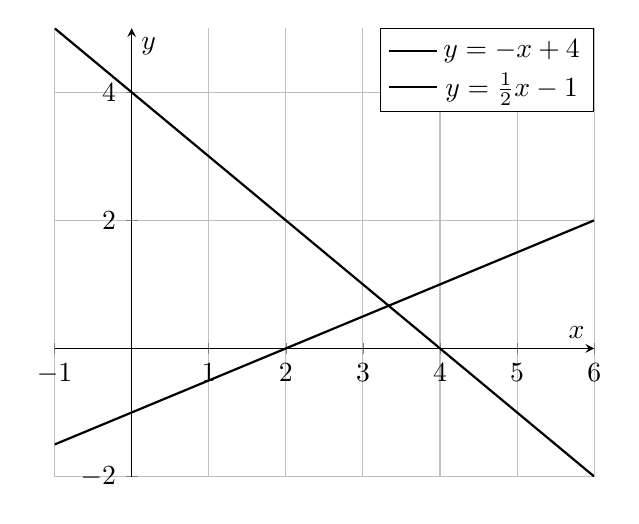
\begin{tikzpicture}
\begin{axis}[
axis lines=middle,
xmin=-1, xmax=6,
ymin=-2, ymax=5,
grid=both,
xlabel={$x$},
ylabel={$y$},
legend style={at={(1,1)}, anchor=north east}
]

% Recta 1
\addplot[domain=-1:6, thick] {-x + 4};
\addlegendentry{$y = -x + 4$}

% Recta 2
\addplot[domain=-1:6, thick] {0.5*x - 1};
\addlegendentry{$y = \frac{1}{2}x - 1$}

\end{axis}
\end{tikzpicture}
\end{center}

\begin{enumerate}
\item Represente en la gráfica la región solución de cada inecuación.
\item Identifique y sombree la región solución del sistema de inecuaciones.
\item Describa brevemente cómo determinó la región solución.
\end{enumerate}